\documentclass[final,11pt]{article}
\usepackage{times}
\usepackage{epsfig}
\usepackage{multirow} 
\usepackage[left=.80in,top=.85in,right=.80in,bottom=.85in]{geometry}
% 14.5 pages:
% \usepackage[left=.78in,top=.74in,right=.78in,bottom=.75in]{geometry}
% lots of margin:
% \usepackage[left=1.00in,top=1.00in,right=1.00in,bottom=1.00in]{geometry}
\usepackage{subfig}
\usepackage{wrapfig}
\usepackage{enumerate}
\usepackage{afterpage}
\usepackage{sectsty}
\usepackage{enumitem}
\usepackage{colortbl} 
\usepackage{comment}
\usepackage{graphicx}
\usepackage{setspace}
%\usepackage{bibspacing}
\usepackage{url}
%\usepackage{gensymb}
%\usepackage{pgfgantt}
\usepackage{amssymb}
\usepackage{nicefrac}

\newif\ifcmm
\cmmfalse
\long\def\CMM#1{
\ifcmm #1\else\relax\fi}
\def\thechapter{./}
\usepackage{moreepsf}
\long\def\AuthorNote#1{%
{\Large\bf #1}}
\def\Action#1{\texttt{#1}}
\def\TiC{{\sc corc}}

\definecolor{purple}{rgb}{.6,.2,.4} 
\definecolor{ltblue}{rgb}{.6,.6,1}

\newcommand{\ignore}[1]{ }
\graphicspath{{./}{figures/}} 

\newcommand{\defn}[1]{\textbf{\textit{#1}}}
\renewcommand{\emph}[1]{\textbf{\textit{#1}}}

% Shrink space in enums and lists
\setlist{topsep=3pt,itemsep=3pt,parsep=3pt}
\setlist[1]{labelindent=\parindent}

% Bolded figure captions in the ACM style
\makeatletter
\long\def\@makecaption#1#2{%
   \vskip 10\p@
   \setbox\@tempboxa\hbox{{\bf#1: #2}}%
   \ifdim \wd\@tempboxa >\hsize
    {\bf #1: #2}\par
     \else
       \hbox to\hsize{\hfil\box\@tempboxa\hfil}%
   \fi}
\makeatother


% Make bullet list singled spaced
\newenvironment{packed_item}{
\begin{list}{\labelitemi}{%
  \leftmargin=1.0em
  \setlength{\itemsep}{3pt}
  \setlength{\parskip}{0pt}
  \setlength{\parsep}{3pt}
}
}{\end{list}}

\def\paragraph#1{%

\smallskip

\noindent{\bf #1}\hbox to 1em{\hss}%
}

\newenvironment{rquote}{\setlength{\leftmargini}{1em}\setlength{\leftmarginii}{1em}\quotation\noindent}{\endquotation}

% Make enumberated list singled spaced
\newenvironment{packed_enum}{
\begin{enumerate}
  \setlength{\itemsep}{1pt}
  \setlength{\parskip}{0pt}
  \setlength{\parsep}{0pt}
}{\end{enumerate}}



% Modify the default section and subsection headers
\makeatletter
\def\@seccntformat#1{\@ifundefined{#1@cntformat}
{\csname the#1\endcsname\,}
{\csname #1@cntformat\endcsname}
}
\def\section@cntformat{\thesection.\,}
\def\subsection@cntformat{\thesubsection.\,}
\def\subsubsection@cntformat{\thesubsubsection.\,}

%phjones changed to 1, 2, 2.1 ...
%\def\thesection{\Roman{section}}
%\def\thesubsection{\thesection.\Alph{subsection}}
%\def\thesubsubsection{\thesubsection.\arabic{subsubsection}}
%\makeatother

%phjones changed to 1, 2, 2.1 ...
\def\thesection{\arabic{section}}
\def\thesubsection{\thesection.\arabic{subsection}}
\def\thesubsubsection{\thesubsection.\arabic{subsubsection}}
\makeatother

\sectionfont{\normalsize\MakeUppercase}
\subsectionfont{\normalsize}


% Create a non-indented bolded start to a paragraph.
\newcommand{\npara}[1]{\noindent{\bf #1}}


% Increase the space between paragraphs.
\setlength{\parskip}{.8ex plus 0.5ex minus 0.2ex} 


%for comments
\newcommand{\FIXME}[1]{\textcolor{red}{FIXME: #1}}

\pagestyle{empty}
\begin{document}
\thispagestyle{empty}
\setcounter{page}{0}

\begin{center}
{\Large Collaborative Research: PPoSS: Planning: Scalable Streaming\\and Cyber-physical Systems}

\vskip 0.2in
{\sc Roger Chamberlain, Jeremy Buhler, Ron Cytron, Chandler Ahrens, Chris Gill}
\\Dept. of Computer Science and Engineering
\\McKelvey School of Engineering
\\and
\\Sam Fox School of Design \& Visual Arts
\\Washington University in St.~Louis
\vskip 0.05in
{\sc Shirley Dyke}
\\Lyles School of Civil Engineering
\\Purdue University
\vskip 0.05in
{\sc Martin Herbordt}
\\Dept. of Electrical and Computer Engineering
\\Boston University
\vskip 0.05in
{\sc Miriam Leeser}
\\Dept. of Electrical and Computer Engineering
\\Northeastern University
\vskip 0.05in
{\sc Anthony Skjellum}
\\Dept. of Computer Science and Engineering
\\University of Tennessee at Chattanooga
\vskip 0.05in
Email: roger@wustl.edu


\end{center}

\clearpage
\pagestyle{plain}
\setcounter{page}{1}
\pagenumbering{arabic}

\section{Introduction}
\label{sec:intro}

Streaming data is a computational paradigm that has broad applicability.
From IoT-derived sensor data streams, to large-scale simulations of physical
systems, to big data being analyzed as part of business practices, it is common
to express the desired computation in terms of one or more streams of data.
In many cases, the performance is critical to the operational success of these
computations, yet the measure of performance varies across disciplines.
While throughput (data elements processed per unit time) is almost always
important, more and more applications have latency constraints as well.

An emerging category of computation that has both a need for scale and
strict latency requirements is cyber-physical systems (CPS). Here, sensor
data (often measuring some aspect of the physical world), is streamed
into the front end of a computational pipeline, individual stages of the
pipeline perform portions of the computation, and the output data
stream represents
commands to actuators that impact/control the physical system.
An example of this type of system is real-time hybrid simulation
experiments in earthquake engineering~\cite{RTHS}, where a computational model
of most of a bridge or building's dynamics in response to an earthquake
ground motion is computed in real-time at millisecond time-scales and is
integrated in-the-loop with sensors, actuators, and control computations
for a physical device (e.g., energy dampers) or specimen (e.g., an
experimental design for part of the structure).

In this plannning grant proposal, we plan to target streaming data 
applications at scale, particularly focusing on those that include explicit
real-time requirements, spanning the range from hard to soft (probabalistic)
latency specifications. We will
investgate mapping of computational needs to execution platforms,
scheduling of both computation and communications, and resource
management algorithms and mechanisms.

In the modern world, where Moore's Law is slowing down~\cite{Waldrop16}
and Dennard scaling has effectively halted~\cite{Bohr07},
computational accelerators are receiving increased 
attention as approaches to improved performance.  In our investigations,
we will explicitly explore the effectiveness of different accelerator
technologies, in particular both Field-Programmable Gate Arrays (FPGAs)
and Graphics Processing Units (GPUs), as execution platforms.

In the current state of the art we've been able to execute the above
example simulations for structures
on the scale of a 9 story building, and only for linear behavior of the
structure -- the objective of our proposed research would be to scale up
significantly to include larger structures, non-linear behavior due to
impacts or damage, and combining finite element models of the structure
with fluid dynamics models for impinging forces (e.g., for a
tsunami/earthquake combination such as occurred in 2011 off Tohoku and
impacted the nuclear reactor at Fukushima).

To enable those kinds of capabilities, we envision scaling from a single
node with tens of computational units to tens to hundreds of nodes with
hundreds of computational units each. Although this is not an extremely
large scale in the world of say high-performance computing, in the realm
of cyber-physical systems it is of very large scale, especially with
respect to operating at millisecond time-scales (or faster, when possible)
and enforcing strict timing guarantees for all sensing and actuation to
ensure control stability and system safety.

To manage the necessary trade-offs among power density and computational
density this will entail, we envision leveraging heterogeneous
architectures harnessing multi-core general purpose processors, FPGAs, and
GPUs in each node, and integrating tens to hundreds of such nodes through
appropriate scheduling and other forms of coordination at the operating
system, concurrency platform, and application levels both locally and
end-to-end.

\FIXME{RC: talk about second application that is a bit less CPS focused, so
we get the overall scope of the proposal in reader's minds.}

\FIXME{RC: below are just random thoughts at this point. Suggestions for
alternatives are definitely welcome.}

Focus areas for proposal:
\begin{enumerate}

\item {\bf Cyber-physical Systems} -- this one is not listed in the call, so we
will have to make the case for its existence.  Chris Gill has ``commensurate 
experience'' (this is the term used in the call.

\item {\bf Computer Architecture} -- this one (and the remaining ones) all are
explicitly listed as candidate focus areas in the call.  Roger Chamberlain has
commesnsurate experience.

\item {\bf Programming Languages and Compilers} -- Ron Cytron is our
champion in this area.

\item {\bf Systems} -- as distinct from cyber-physical systems, we are
calling this a focus relating to more classic systems software (e.g., OS,
middleware, development environments, networks, etc.).  Jeremy Buhler can be called
our expert here. I'm putting Martin Herbort and Tony Skjellum here as well,
until they tell me they would prefer to be identified with another area.

\FIXME{RC: Martin and Miriam, look over the NSF call and let me know which
``focus area'' where you feel most comfortable being included.}

\end{enumerate}
\section{Driver Applications}
\label{sec:apps}

\FIXME{RC: The text below is mostly from~\cite{cag18}.}

\subsection{Real-Time Hybrid Simulation of Civil Structures}

Our first cyber-physical application example comes from the domain of
\emph{real-time hybrid structural} (RTHS)~\cite{RTHS} experiments used in
structural and earthquake engineering.  In these experiments, a physical
specimen is connected to a low-level control loop via sensors
that can measure the position and/or acceleration of the specimen continuously,
communicate those measurements frequently as digital readings through a DAQ
board, and in turn receive and apply commands sent by the low-level
controller through the DAQ board to actuators that are also connected to
the specimen.  Low-level control design includes both the dynamics of
the specimen and compensation for the dynamics of
the actuators to ensure that appropriate forces are applied to the specimen
over time. The sensor measurements are used as inputs to a simulation
(e.g., using a finite element model) that computes the behavior of the overall structure,
including the next set of forces to apply to the specimen at the next time step.  Within
each iteration, both the low-level control loop and the simulation must complete within a
millisecond or less to avoid losing high-frequency vibrations or other behaviors
of the specimen.

Figure~\ref{fig:rths} shows a scale-model version of such an experiment, at
Washington University in St. Louis.  Full-scale experiments require hydraulic
actuators and other capabilities found in facilities such as the Bowen Laboratory
at Purdue University, and our experiences working with both versions has shown
that scale-model experiments offer a useful setting for designing, developing, and
debugging cyber-physical experiments before moving them to the full-scale setting.
\FIXME{RC: add picture of full-scale system at Purdue.}

\begin{figure}[ht]
\centering
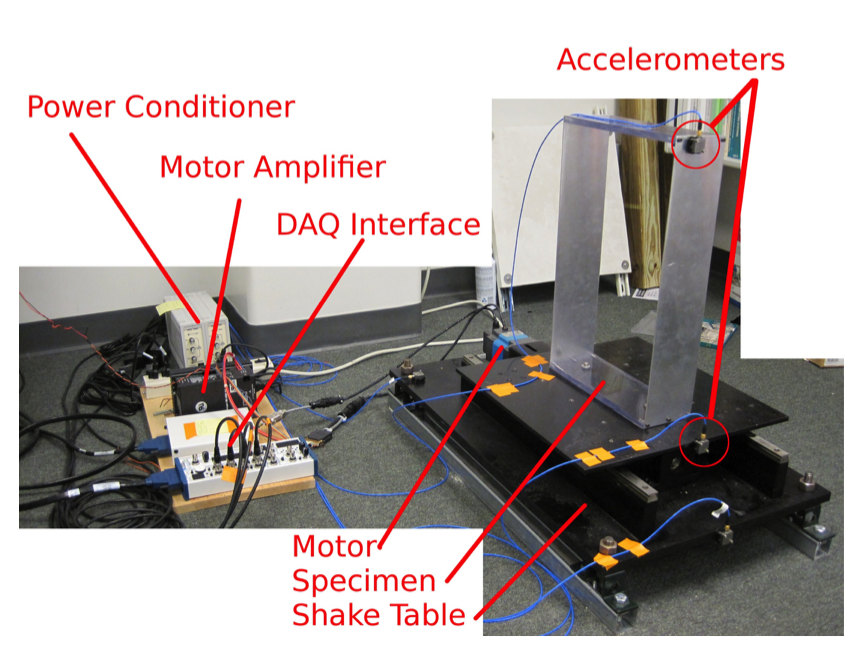
\includegraphics[width=0.5\columnwidth]{rths}
\caption{RTHS experiment at Washington University in St. Louis.}
\label{fig:rths}
\end{figure}

Higher-level objectives include the ability to substitute simulated versus physical versions
of different parts of a structure~\cite{Huang10}, and through advances in
parallel real-time concurrency platforms to trade-off computational demand and
time scales~\cite{Ferry14} allowing resources to be concentrated for portions of
the structure that are most significant.

\FIXME{RC: we need to let the reader know that this is a finite-element model, and
point out that \emph{lots} of other applications use finite-element models of some
aspect of the physical world.}

\FIXME{RC: tie this into the research questions we address later.}

\subsection{Catoptric Systems}

Figure~\ref{fig:amp} shows a prototype catoptric (mirror) surface
called \emph{AMP} that was
designed, fabricated, and installed during an undergraduate architecture studio
taught by Co-PI C.~Ahrens. The installation redirects light from gable ends of an
existing building into the darker recesses of the atrium
to create better natural lighting where it is desired.
We next developed a
new version in which over 600 mirrors are under
active, 2-axis control and therefore the mirrors
can be pointed in different directions dynamically as desired over
time~\cite{acmbg19,acmb18,cagm18}.
This next-generation installation is within
the south wall of the Steinberg Hall atrium on the campus of
Washington University; a subset of the mirrors in this new
installation is shown in Figure~\ref{fig:steinberg}.

\begin{figure}[ht]
\centering
\subfloat[\mbox{ }]{
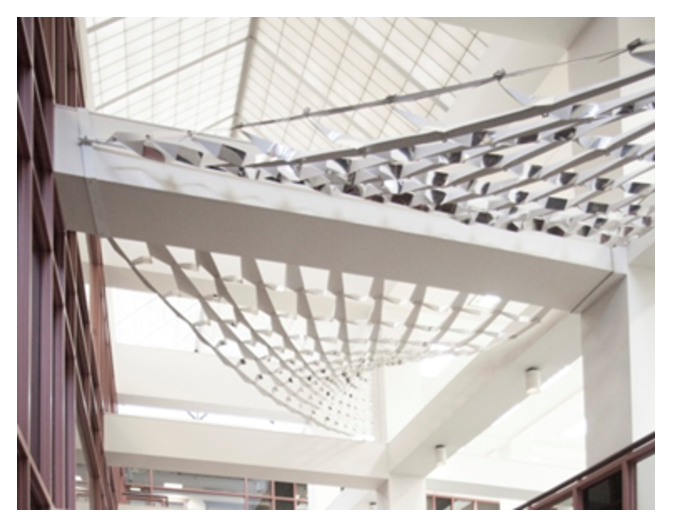
\includegraphics[width=0.43\linewidth]{amp}
\label{fig:amp}}
\quad %\qquad
\subfloat[\mbox{ }]{
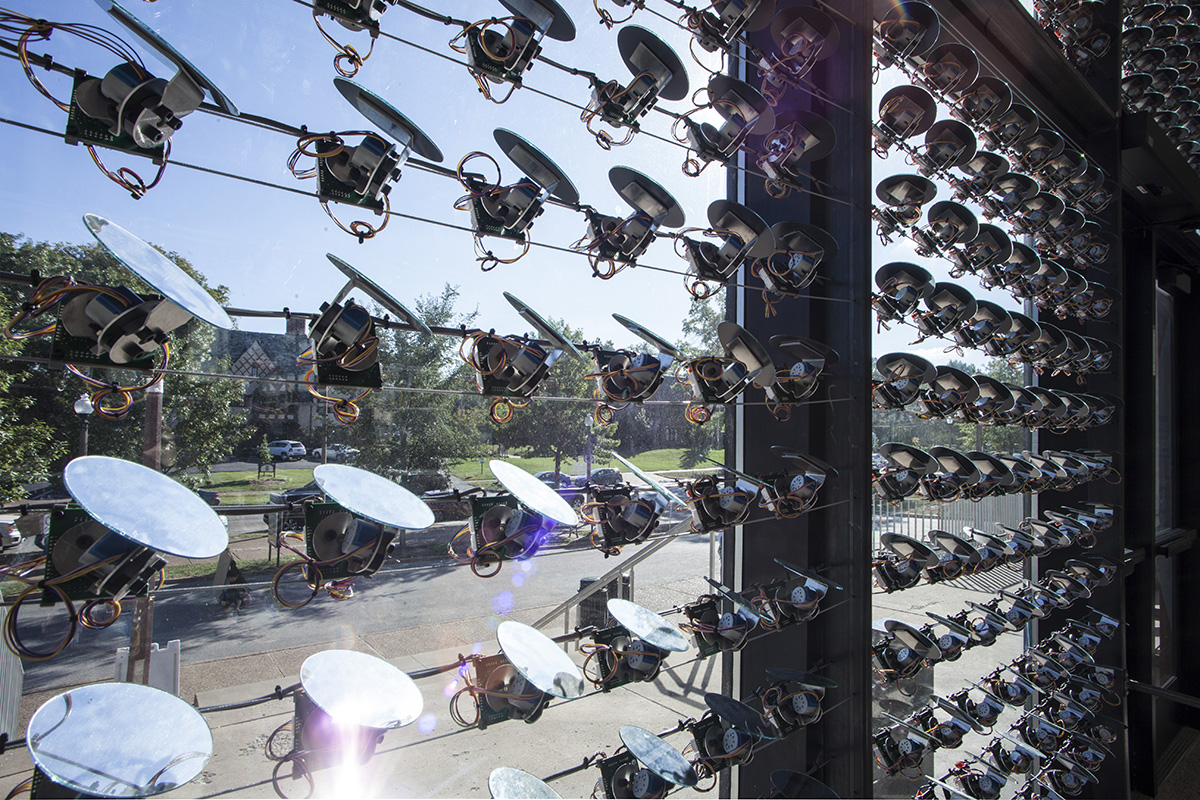
\includegraphics[width=0.5\linewidth]{CS_prototype_012_sm}
\label{fig:steinberg}}
\caption{Catoptric system prototypes.
(a)~\emph{AMP}, TRex building, St.~Louis.
(b)~Steinberg Hall, St.~Louis.
}
\label{fig:proto}
\end{figure}


Using ray tracing algorithms and straightforward low-level control mechanisms,
we can position a set of mirrors to direct light where it is desired. The
high-level decisions revolve around the questions of, ``how do we operate
the system safely?'' and, ``where do we want the light to be?''
The first question relies on feedback obout the actual configuration of the system.
One feedback mechanism we will use is visual data (imagery and video). This
will include determination of the true orientation of each mirror, providing information
on the available light and its current positioning, as well well as providing feedback
on benefits accrued.

The second question becomes even more interesting if we expand the
higher level options to include varying the intensity of daylight that is
directed into an area according to the area's use (e.g., lower to improve
contrast when computer screens are being used, or higher when people are
reading paper materials), or the ability to direct incoming sunlight that
is not needed for another purpose into a heat exchanger that can harvest
energy for the building's HVAC system.  Given a bounded resource
(currently available sunlight), we now are charged
with balancing the relative benefits of natural sunlight illumination within
a physical space vs.~the harvesting of thermal energy which can potentially
reduce operating costs for that same physical space.

Data are streaming from the sensors providing feedback, as well as the users'
directions for use of the available light.  Especially for safety concerns, the
latency constraints for processing this data stream and making decisions are
strict.  Also, for the Steinberg prototype, several of the communications
between computational elements are via wireless links.  Neither best effort computation
nor communication will be sufficient. Guarantess are needed.

\section{Research}
\label{sec:research}

\FIXME{RC: What the heck are we proposing to actually do? And how to we plan for it? Remember, this is a proposal for a planning grant.}

\FIXME{RC: The focus is on incorporating latency constraints on streaming data computations for cyber-physical systems as they scale up.}

\FIXME{RC: This will include scheduling of computational loads across ``cores'' and ``nodes'' (both terms need to be defined), and enabling communications between nodes (cores are assumed to have a common memory system).}

\subsection{General Questions}

\FIXME{RC: All of the following in the whole section is speculative at present. One could make a credible case that all of the points in this subsection really need to have been made already in the introduction, and don't warrant repeating here.}

When deploying a streaming computation on heterogenous highly-parallel systems, the primary questions that must be addressed include:

\begin{itemize}

\item What are the admission control mechanisms to ensure that latency (and other) requirements are met?

\item What compute stages get mapped to which specific execution platforms (both type and identification)?

\item What communications paths are allocated to move data? Remember, we know a lot about the application's communication
topology at compile time (unlike the general case that has to be dealt with by MPI).

\item What scheduling algorithms (for both computation and communication) are effective?

\item Are there other ``high-level'' general questions, or does the above cover it?  

\end{itemize}

\subsection{Specific Research Focus}

\FIXME{RC: Here, we need to articulate the specific ideas and directions that will be pursued.  We have some leeway here, given the fact
that this is a planning grant, but we do need to impress reviewers, so we can't give ourselves too much leeway to be wishy-washy.}

The following things will receive attention (they are in no particular order):

\begin{itemize}

\item How do we express latency requirements?  Both hard real-time and soft real-time (the two will be different).

\item What formal models can we leverage/develop that let us prove properties of the mapping/scheduling algortihms that we propose? Here I'm thinking of both CPS-style models that speak to schedulability of real-time computations and the kinds of models we've used for deadlock avoidance in streaming computations and correctness in MERCATOR.

\item Scale up MERCATOR to multiple GPUs.

\item Use of bump-in-the-wire FPGAs to facilitate communications functions (both wired and wireless).

\item Use of bump-in-the-wire FPGAs to perform relevant pipeline stage computations.

\item What else should we include (I'm pretty tired as I'm writing this, so I probably am forgetting something pretty major!)?

\end{itemize}

\subsection{Experimental Validation}

The research ideas that ultimately get pursued must be evaluated for both correcness and effectiveness.  While formal methods are sufficient to show correctness of some of the theoretical results (e.g., schedulability analysis), the bulk of the evaluation will requre physical experimentation and assessment of empirical data.  Ultimately, we will build prototype systems to test our ideas, and evaluate these prototypes to judge their effectiveness.

The core of our experimental infrastructure is comprised of three resources, each of which is described in more detail in the Facilities section of this proposal.  The first two elements are tied to our two application drivers: real-time hybrid simulation and catoptric systems.
Physical shake tables are extant at both Washington Univ. in St. Louis (see Figure~\ref{fig:rths}) and Purdue Univ. (see Figure~\ref{fig:rthsbig}). An experimental catoptric system is in place at Washington Univ. (see Figure~\ref{fig:steinberg}).

The thiird resource that will be leveraged to support this work is the Open Cloud Testbed (OCT) installed at the Massachusetts Green High-Performance Computing Center (MGHPCC) near Boston. Both Dr.~Herbordt of Boston Univ. and Dr.~Leeser of Northeastern Univ. are Co-PIs on the NSF-funded OCT, and PI Chamberlain is a member of the OCT's Technical Advisory Board. An important element of the OCT is the inclusion of FPGAs in a number of the testbed compute nodes, making bump-in-the-wire FPGA nodes available in a way that will support the kinds of experimental evaluations we anticipate.  Both the compute nodes and associated FPGAs will be reservable in a (near) bare-metal allocation that will allow for almost unlimited experimental opportunity.
\section{Planning Activities}
\label{sec:plan}

This proposal represents a collaboration that includes \FIXME{9 or 10} senior personnel across \FIXME{4 or 5} institutions. This implies that the coordination effort will be significant, and will not happen without intentionality.  We will initiate the project with in in-person meeting to be held prior to the spring semester for each of the institutions (i.e., right after the beginning of the 2021 calendar year). The purpose of this initial face-to-face meeting will include the following:
\begin{itemize}

\item Ensure that each individual gets to know all other individuals. We will have the PI from each institution give a short (informal) presentation to the rest of the group that both provides background on the strenghts that each institution brings to the table and promotes the general notions that are to be the focus of the research effort.

\item Provide the opportunity for free-form brainstorming. While this planning proposal articulates some of the notions that will be pursued ultimately, given the nature of research the thinking of the participants will surely have evolved. We desire that the planning activities are ultimately targeting our very best research ideas.

\item Identify and provision for the preliminary results that we feel are necessary to credibly make the case that our research ideas are credible. What preliminary work needs to be done, and how will we see that it is accomplished?

\item Finalize the plans for regular meetings, feedback, and ultimate decisions for research direcition.

\end{itemize}

The outcome of this initial face-to-face meeting will include both a near-term plan for further interactions (primarily to be arranged via remote communication) and for action items for each of the participants.
\section{Broader Impacts}
\label{sec:broader}

\FIXME{RC: say something about how what we are doing is important in
areas beyond our particular driver applications.}

We are committed to promoting diversity and will seek opportunities to
involve students from underrepresented groups in this project.
We will leverage a pair of existing university programs to help us
attract students from traditionally underrepresented groups.  The Olin
Fellowship Program (for women) and the Chancellor's Fellowship Program
(aimed at African-American students) have had a successful track
record of enabling individuals to pursue graduate study.  In our
experience, the most effective method for attracting students from
underrepresented groups is by personal contact with a suitable role
model.  To facilitate this, we regularly ask the appropriately
qualified individuals in our group to be actively involved in the
recruiting process.  This cohort currently includes two female
faculty and one minority (African-American)
graduate student.

\FIXME{RC: I'm always open to new ideas of things we could do in
this area.  Given that this is a planning grant, we'd of course really be
talking about the eventually funded research grant.}
\section{Results from Prior NSF Support}
\label{sec:prior}

Faculty Co-PI C. Ahrens has not had prior NSF funding.
The projects described
below are representative examples of NSF-supported research led by PI 
R.~Chamberlain and the remaining senior personnel.

%\noindent
{\bf CSR: Small: Concurrent Accelerated Data Integration}
{\bf (CNS-1527510,
PI R. Chamberlain, Co-PI R. Cytron)} and
{\bf CSR: Medium: Performant Architecturally Diverse Systems via Aspect Oriented Programming}
{\bf (CNS-1763503, PI R. Chamberlain, Co-PIs J. Buhler and R. Cytron)}, 
10/2015--9/2019 and 9/2018--8/2022, \$519,275 + \$1,214,675. 
%
\textbf{Intellectual Merit} -- This project is investigating the
accelerated execution of streaming applications and data integration workflows, which
increasingly are bottlenecks in data science. Execution platforms
include both graphics engines and FPGAs.
%
\textbf{Broader Impacts} -- This project has supported 5
graduate and 6 REU students.  The applications investigated
come from biology, astrophysics, and the IoT,
further expanding the scope of the students'
experience.
%
\textbf{Evidence of Research Products and their Availability} --
Publications resulting from this work include~\cite{cc19,ccb19,dibs,c17,fcbmc19,mgc16,js16}.
A benchmark suite of the data integration workflows has been released
as a community resource~\cite{dibsv1}.

%\noindent
{\bf CPS: Medium: Collaborative: CyberMech, a Novel Run-Time Substrate for 
Cyber-Mechanical Systems}
{\bf (CNS-1136073 and CNS-1136075,
WU PI C. Gill, Purdue PI S. Dyke)}, 9/2011-8/2016, \$1,800,000 total.  
%
This research project developed novel foundations for parallel real-time computing, demonstrating the first ever real-time hybrid simulation involving a thousand-degree-of-freedom structure at millisecond time scales.
%
\textbf{Intellectual Merit}~-- Results of this research include new methods for parallel real-time execution of control and simulation computations, new parallel real-time scheduling techniques and analyses, and characterization and exploitation of trade-offs involving both high computational demand and stringent timing constraints.
%
\textbf{Broader Impacts}~-- This multi-university project involved 7 PhD, 3 masters, and 7 undergraduate students, and 2 visiting scholars in highly multi-disciplinary research collaborations.  Results of this research are spurring
further advances in parallel real-time computing and natural hazards
engineering.
%
\textbf{Evidence of Research Products and their Availability}~-- Results of
this 
collaborative research appeared in 10 publications at
top-tier conferences and journals.
Data, experiment configurations, platform software, and simulation source-code 
have been published on-line.

\FIXME{RC: need to include projects from Martin and Miriam.}

\clearpage
\bibliographystyle{abbrv}
\bibliography{prop}

\end{document}
